\documentclass[titlepage]{article}
\usepackage{graphicx} % Required for inserting images
\usepackage{enumitem}

% Setup for listing functional requirements
\def\threedigits#1{% 
\ifnum#1<100 0\fi 
\ifnum#1<10 0\fi 
\number#1}

\title{Job Search Engine: Software Requirements Specification}
\author{
    Chris Pappelis\\
    cfp4@hood.edu
    \and
    Matthew Smith\\
    mps3@hood.edu
}
\date{February 11, 2025\\Spring 2025}

\begin{document}

\maketitle

\section{Introduction}

\subsection{Purpose}
The purpose of the Job Search Engine\footnote{``Job Search Engine'' is a tentative name; a more appropriate name shall be decided upon later in the course of development.} is to make finding employment in computer science occupations simpler while showing the user what skills and tools they should learn to make themselves more applicable to employers in their region.

\subsection{Intended Audience}
The intended audience of the Job Search Engine is people in computer science or related fields looking for employment and/or wanting to strengthen their r\'esum\'e. This includes both students and established members of the computer science field. The system will be accessible to the public and shall be designed for a general audience.

\subsection{Intended Use}
The intended use of the Job Search Engine is to assist those entering or currently working in the computer science field with finding jobs that best match their skill sets, or determining which skills they need to learn or master in order to qualify for their desired jobs and strengthen their r\'esum\'e.

\subsection{Scope}
The system only considers computer science-related occupations within the United States of America. The system shall include a modest sample of jobs scraped from the web; such a sample will not encompass all jobs available at the time of viewing. The main goals of the Job Search Engine are to help those in the tech field find jobs they are most likely to be accepted for and provide an accurate overview of skills that employers in the tech field are looking for.

\subsection{Definitions and Acronyms}

\begin{itemize}
    \item \textbf{Choropleth map}: A geographical map in which the colors of regions are used to indicate a data value in that region.
    \item \textbf{Web scraper}: A computer program that extracts data from websites.
\end{itemize}

\section{Overall Description}

The Job Search Engine is a web app for finding jobs and discovering in-demand skills by employers in computer science and adjacent fields. The app will provide three central functions: finding the jobs most compatible with a user in a certain region, finding the skills that are most in-demand by employers in a certain region, and giving a logged-in user a summary of jobs and skills in their region at a glance. These functions come in the form of the job search, skill search, and dashboard, respectively.

\subsection{User Needs}

The user will need accurate compatibility scores for jobs, easy-to-read and informative visualizations of job skill data, intuitive search functions to view data and find jobs, and easy access to original job postings should they want to apply.

\subsection{Assumptions and Dependencies}

\subsubsection{Assumptions}

\begin{itemize}
    \item The system assumes that job data from Indeed or other job listing services will be freely and legally available.
    \item The system assumes that all job postings will have an associated description from which to extract data.
    \item The system assumes that the user will have basic computer and Internet literacy.
\end{itemize}

\subsubsection{Dependencies}

\begin{itemize}
    \item The system will use the JobSpy library for Python to handle scraping job listings.
\end{itemize}

\section{System Features and Requirements}

\subsection{Functional Requirements}

\begin{enumerate}[label={\textbf{FR\protect\threedigits{\theenumi}}}, leftmargin = *]
\subsubsection{Job Data}
    \item The system shall use a web scraper to retrieve job posting data, including job titles, descriptions, locations, posting dates, and salaries, from at least one job posting website.
    \item The system shall extract, from each scraped job posting, the skill, education, and experience requirements mentioned in the job description.
    \item Skill requirements extracted from jobs shall include programming languages (e.g., Java, C, Python), frameworks (e.g., Django, Angular), and database tools (e.g., MySQL, MongoDB).

\subsubsection{Job and Skill Search}
    \item The system shall provide a search form for jobs wherein users enter their skills, education, years of experience, and location to search for jobs.
    \item In a job search, the system shall generate, for each job, a compatibility score between 0 and 100 based on the skills, education, and experience entered by the user.
    \item In a job search, each job shall have a link to the official posting of the job on an external website.
    \item The system shall provide a search form for skills wherein users enter a U.S. state to find in-demand skills in that state.

\subsubsection{Visualization}
    \item In a skill search, the system shall generate visualizations of in-demand skills in a selected U.S. state.
    \item In a skill search, skill data shall be visualized in a bar chart, in which the $y$-axis will represent the number of job descriptions that mention a skill, and the $x$-axis will represent different skills.
    \item In a skill search, skill data shall be visualized in a choropleth map broken down by county, in which the color of a county represents the most in-demand skill in that county.

\subsubsection{Dashboard}
    \item The system shall have a dashboard containing job and skill analytics relevant to the user.
    \item The dashboard shall contain a bar chart showing the most in-demand skills in the user's state.
    \item The dashboard shall present skill data using a choropleth map broken down by county, in which the depth of the color of a county represents how in-demand the skill is. Skills may be dynamically changed using a drop-down menu.
    \item The dashboard shall contain a list of the top 10 most compatible jobs for the user based on their compatibility scores, with a link to show more jobs, which redirects the user to a job search.
    \item The dashboard shall not display any tailored data visualization or jobs if the user is logged out.

\subsubsection{User Account Management}
    \item A user shall be able to create an account with a unique username and a password.
    \item A user shall be required to choose which U.S. state they live in during account creation.
    \item A user shall be able to enter the following information during account creation: a variable number of skills chosen from predefined options, an education level chosen from predefined options, and a number of years of experience in the field.
    \item A user shall be able to log in to their account using their username and password.
    \item A user shall be able to add and delete skills from their account.
    \item A user shall be able to edit their education level, years of experience, and location.
\end{enumerate}

\subsection{External Interface Requirements}

\begin{itemize}
    \item The system will communicate with a database back-end to retrieve user and job data.
    \item The system will be accessed through a web browser.
\end{itemize}

\subsection{System Features}

\begin{itemize}
    \item \textbf{Web scraper}: Job data will be scraped from job posting websites using a web scraper. Data gathered will include job titles, descriptions, locations, posting dates, and salaries, if applicable.
    \item \textbf{Skill extraction algorithm}: The system will include an algorithm that, given a job's description, can extract a list of skills mentioned in the description as well as the prerequisite years of experience and/or education necessary for the job.
    \item \textbf{Data visualization}: Data extracted from jobs will be visualized in several ways. Visualizations include choropleth maps and bar charts.
    \item \textbf{Compatibility score algorithm}: The system will include an algorithm that, given a job's skill data extracted from the description and the user's skill, education, and experience data, generates a score from 0 to 100 based on how many of the requirements the user meets. The higher the score, the more qualified the user is for the job.
    \item \textbf{User account system}: Users will be able to create an account with a username and a password and enter their skills, education, years of experience, and location for a more tailored experience. Benefits of creating an account include access to a dashboard that includes data on jobs and skills in their region.
\end{itemize}

\begin{figure}
    \centering
    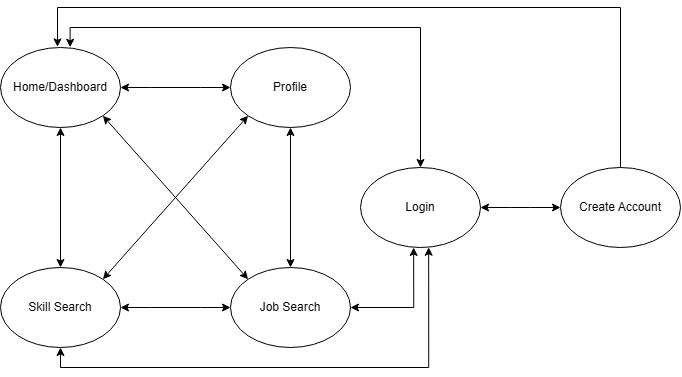
\includegraphics[width=1\linewidth]{WebsiteStateDiagram.png}
    \caption{State diagram of the front-end of the Job Search Engine. Each node represents a webpage. A double-sided arrow between two nodes shows that direct navigation is possible between the two pages. A single-sided arrow shows that direct navigation is only possible in one direction.}
    \label{fig:state_diagram}
\end{figure}

\subsection{Nonfunctional Requirements}

\begin{enumerate}[label={\textbf{NFR\protect\threedigits{\theenumi}}}, leftmargin = *]
    \item The system's repository of jobs shall contain data from no less than 5000 jobs.
    \item The system shall be designed to scale as the number of job postings in the repository increases.
    \item The system shall provide a response to user searches for jobs or skills within no more than three seconds.
    \item The system shall be fully usable on popular desktop web browsers including Google Chrome, Firefox, and Microsoft Edge.
    \item The system shall be usable by a general audience with minimal training.
    \item User password data shall be securely stored using encryption.
\end{enumerate}

\end{document}
